\chapter{Challenges for Implementation}
Tracking users with gesture-based technology is one thing, interpreting whether the intended function is meant in another thing. Intent and context is integral to human interaction and especially when using gestures. Intent and context is a very important part of gesture technology moving forward.

\section{Voice Controls}
\subsection{Context and Intent}

\begin{wrapfigure}{r}{0.5\textwidth}
  \begin{center}
    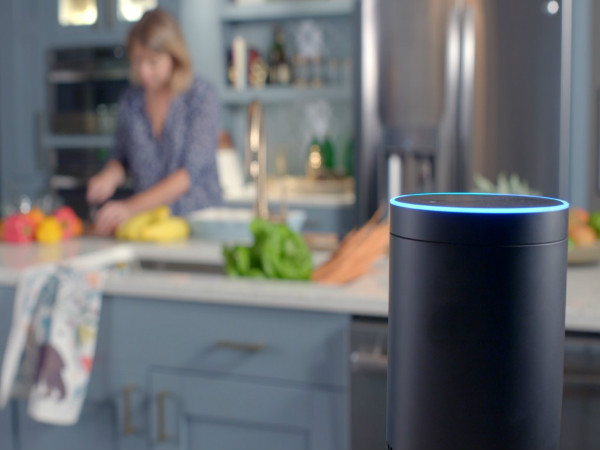
\includegraphics[width=0.48\textwidth]{img/alexa.jpg}
  \end{center}
  \caption{Alexa Active}
\end{wrapfigure}

A big problem with voice controls is interpreting whether the user is trying to enact a function or the user is just talking to another person. Alexa, for example, will commonly mistake the two people talking about Alexa for them trying to interact with the device. The Alexa machine has difficulty understanding the context of the conversation and activates when hearing the keyword being spoken. This keyword is used to activate the device with the remaining speech being the function the user wishes to enact. Manufacturers are still trying to grasp when the user is talking about the device or trying to use it. Basic workaround such as Calling the device Google Assistant and making the wake word 'Hey Google' is a basic workaround which has worked for Google, but failed for Amazon. Amazon customers often complain their home assistant thinks they're trying to use it when they are just talking about it. This is a problem with how Amazon advertised their devices under Amazon Alexa and Alexa Compatible which has caused the user to think of the entire device as Alexa rather than an Amazon Echo with Alexa built in.

\subsection{Interpreting Intent}
Interpreting what the user wants is a hard task. There are many ways of phrasing sentences and figuring out what the user is trying to do is a challenging task.

Devices like Amazon Echo have three major methods of figuring out user intent. Alexa will separate a phrase into three parts.

\begin{itemize}
    \item Intents
    \item Slots
    \item Slot Types
\end{itemize}

The three parts help break down a sentence and figure out what the user wants the device to do. 'Intents' are like functions in programming, 'Slots' are the variables and 'Slot Types' are the variable types. Using these three parts Alexa can break the sentence down and figure out what has to be done. For example, if the user says 'What is one plus two',
Alexa will use the sentence to find an Intent that best matches what the user has asked. Once found Alexa will get the slots in the sentence. The slots are 'one' and 'two'. Alexa will then use slot types to figure out what the slots are. Slot types are numerous ranging from numbers to German cities to American politicians. With the slot type, Alexa can figure out what is being said. Using the slot type in this example Alexa will figure out that 'one' and 'two' are numbers and return '1' and '2' instead of the string representation. Using this method Alexa can figure out most of the user requests.

\section{Physical Controls}

Tracking physical gestures is very tricky because unlike voice gestures there is no wake word to recognize tracking and cease after the function has been enacted. 

\begin{wrapfigure}{r}{0.5\textwidth}
  \begin{center}
    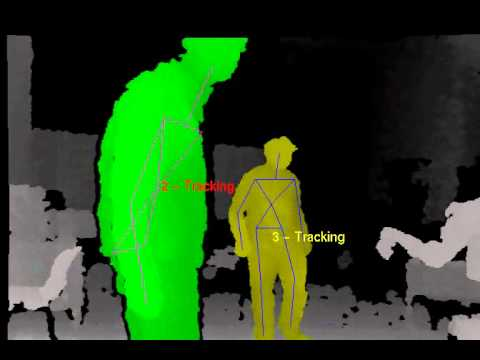
\includegraphics[width=0.48\textwidth]{img/kinecttracking.jpg}
  \end{center}
  \caption{Kinect Tracking}
\end{wrapfigure}

Microsoft's Kinect for example, its tracking works be imposing a digital skeleton onto the users in the frame in order to track location and limb movement. This method makes for accurate tracking of the entire body and can slowly be expanded upon while also being compatible with previous games and applications. 

Microsoft's Kinect is an extremely accurate gesture tracking technology which has been adapted to work in industries beyond its core gaming focus. But its accuracy may cause problems when the user wishes it to stop tracking. Microsoft has come up with multiple ways to fix the problem of gesture tracking when the user wishes to pause the software. The user can do a specific gesture to bring up the Xbox menu in order to pause the game and can use this gesture in order to return to the game. But the main method of interacting with menus and pausing or exiting an application is by using the built-in voice gestures on the Kinect. By using these voice gestures the user can still remain away from any physical input and control any application through gestures. The Kinect can turn on the Xbox console through voice gestures and then can be controlled through gestures both voice and moving your arm.